\documentclass[tikz, border=1mm]{standalone}
\usepackage{tikz} 
\usetikzlibrary{arrows.meta}
\usepackage{pgfplots}

\begin{document}

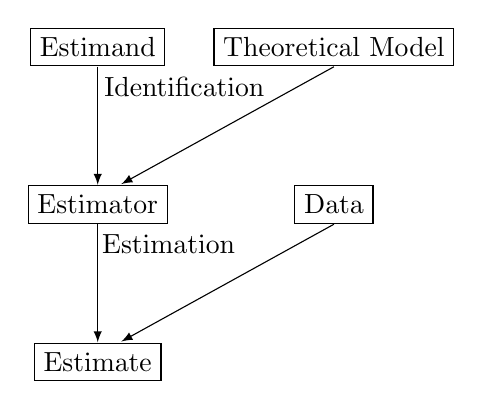
\begin{tikzpicture}
    % nodes
    \node at (0,2) [rectangle,draw]  {Estimand};
    \node at (3,2) [rectangle,draw] {Theoretical Model}; %,fill={black!15}
    \node at (0,0) [rectangle,draw] {Estimator}; %,fill={black!15}
    \node at (3,0) [rectangle,draw] {Data};
    \node at (0,-2) [rectangle,draw] {Estimate};
    \node at (1.1,1.5) {Identification};
    \node at (0.9,-0.5) {Estimation};
        
	% paths
    \draw[-{latex}](0,1.75) to (0,0.25); % Estimand -> Estimator 
    \draw[-{latex}](3,1.75) to (0.3,0.26); % SciModel -> Estimator
    \draw[-{latex}](0,-0.25) to (0,-1.75); % Estimator -> Estimate
    \draw[-{latex}](3,-0.25) to (0.3,-1.74); % Data -> Estimate
    
\end{tikzpicture}

\end{document}
